\Tsec{T13}

Известен дипольный момент земли $\vc{\mu} = 8.1 \cdot 10^{25}$  гаусс$\cdot$см$^3$. Найдём в полярных координатах линии магнитного диполя, и определим, как меняется поле вдоль силовой линии. 


\textbf{Уравнение силовых линий магнитного поля.}
Поле от магнитного диполя $\vc{H}$ можем записать, как
\begin{equation*}
    \vc{H} = \frac{3 \left(\vc{\mu} \cdot \vc{n}\right) \vc{n} - \vc{\mu}}{r^3},
    \hspace{5 mm} 
    \vc{n} = \frac{\vc{r}}{r}.
\end{equation*}
Считая, что $\vc{\mu} = \mu \vc{o}$, и выбирая $Oz \parallel \vc{o}$, можем записать
\begin{equation*}
    \vc{\mu} \cdot \vc{e}_r = \mu_r, \hspace{5 mm} 
    \vc{\mu} \cdot \vc{e}_\theta = \mu_\theta, \hspace{5 mm} 
    \vc{\mu} \cdot \vc{e}_\varphi = \mu_\varphi. \hspace{5 mm} 
\end{equation*}
Также верно, что $\vc{n} = \vc{r} / r = \vc{e}_r$. Можем вычислить все проекции
\begin{equation*}
    \mu_r = \mu  (\vc{o} \cdot \vc{e}_r) = \mu (\vc{e}_z \cdot \vc{e}_r) = \mu \cos \theta,
    \hspace{5 mm} 
    \mu_\theta = - \mu \sin \theta, 
    \hspace{5 mm} 
    \mu_\varphi = 0.
\end{equation*}
Так приходим к записи для векторов в сферических координатах
\begin{equation*}
    \vc{\mu} =  \mu \left(\cos \theta,\, -\sin\theta,\, 0\right)\T,
    \hspace{5 mm} 
    \vc{n}  = \left(1,\, 0,\, 0\right)\T.
\end{equation*}
Тогда магнитное поле
\begin{equation*}
    \vc{H} = \frac{1}{r^3}\mu \begin{pmatrix}
        3 \cos \theta - \cos \theta \\
        - (-\sin \theta) \\
        0
    \end{pmatrix} = \frac{\mu}{r^3} \begin{pmatrix}
        2 \cos \theta \\ \sin \theta \\ 0
    \end{pmatrix},
    \hspace{5 mm} 
    d \vc{l} = \begin{pmatrix}
        dr \\  r \ \theta \\ r \sin \theta \d \varphi
    \end{pmatrix},
    \hspace{5 mm}
    \frac{H_r}{\d l_r} = \frac{H_\theta}{\d l \theta}.
\end{equation*}
Раскрывая последнее уравнение находим
\begin{equation*}
    \frac{d r}{r} = \frac{2 \cos \theta}{\sin \theta}\d \theta = 2 \frac{\d \sin \theta}{\sin \theta},
    \hspace{0.5cm} \Rightarrow \hspace{0.5cm}
    \ln r = 2 \ln \sin \theta + \const,
    \hspace{0.5cm} \Rightarrow \hspace{0.5cm}
    \boxed{
    r(\theta) = r_0 \sin^2 \theta
    }
    , \hspace{5 mm} r_0 = r\left(\theta=\pi/2\right).
\end{equation*}
Можно построить такой бублик (сииметричный относительно оси $z$, или относительно поворота $\varphi$), см. рис. 1.
\begin{figure}[h]
    \centering
    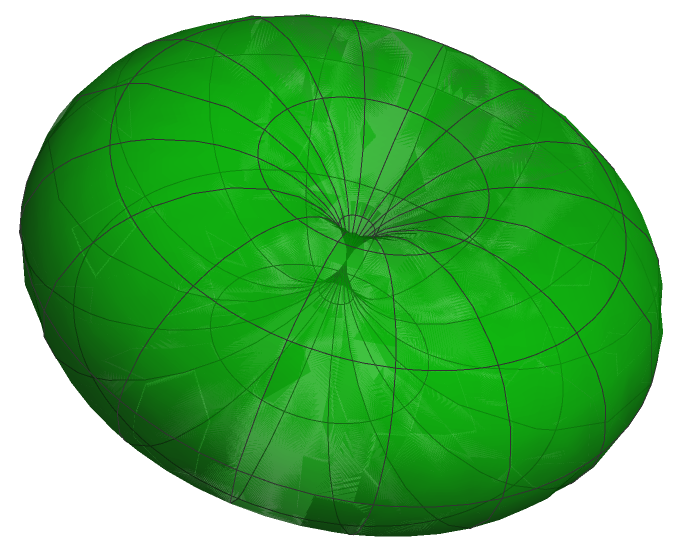
\includegraphics[width=0.3\textwidth]{figures/t13.png}
    \caption{Поверхность, образованная силовыми линиями в задаче 13.}
    %\label{fig:}
\end{figure}


\textbf{Кривизна силовой линии магнитного поля}. Определим $\vc{h} = \vc{H} / H$, для него верно
\begin{equation*}
    \dot{\vc{H}} = \frac{d }{d t}  \left(
        \vc{h}(\vc{r} + \vc{h} \d t) - \vc{h}(\vc{r})
    \right) = \frac{\vc{h}}{\rho} \cdot \vc{h}^2.
\end{equation*}
Расписывая дифференцирование, находим
\begin{equation*}
    \vc{h}(\vc{r} + \vc{h} \d t) - \vc{h}(\vc{r}) = h^\alpha \d t \partial_\alpha \vc{h},
    \hspace{0.5cm} \Rightarrow \hspace{0.5cm}  (\vc{h} \cdot \nabla) \vc{h} = \frac{\vc{n}}{\rho}.
\end{equation*}
Подробнее рассмотрим диффернцирование по направлению
\begin{equation*}
    \vc{h} \cdot \nabla = 
    h_r \partial_r + h_\theta \frac{1}{r} \partial_\theta + h_\varphi \frac{1}{r\sin \theta} \partial_\varphi.
\end{equation*}
Магнитное поле, соответсвенно, равно
\begin{equation*}
    \vc{H}^2 = \left(\frac{\mu}{r^3}\right)^2 \cdot (3 \cos^2 \theta + 1),
    \hspace{0.5cm} \Rightarrow \hspace{0.5cm}
    h_r = \frac{2 \cos \theta}{\sqrt{3 \cos^2 \theta + 1}},
    \hspace{5 mm} 
    h_\theta = \frac{\sin\theta}{\sqrt{\sin^2 \theta + 2}}.
\end{equation*}
Наконец, можем подтсавить их в $\left(\vc{h} \cdot \nabla\right) \vc{h} = \left(
    h_r \partial_r + h_\theta \frac{1}{r} \partial_\theta
\right) \vc{h} = \vc{n}/\rho$. Так, например, на экваторе $\theta=\pi/2$, $h_r = 0$, $h_\theta = 1$:
\begin{equation*}
    \left(
    \frac{1}{r} \partial_\theta
\right) \vc{h} = \frac{1}{r} \partial_\theta \left(
    h_r \vc{e}_r + h_\theta \vc{e}_\theta
\right) \bigg|_{\theta=\pi/2} = \frac{1}{r} \left(
      \partial_\theta h_r \vc{e}_r + h_r \partial_\theta \vc{e}_r + \partial_\theta h_\theta \vc{e}_\theta + h_\theta \partial_\theta \vc{e}_\theta  
\right).
\end{equation*}
В частноcти, слагаемые равноы
\begin{align*}
    \partial_\theta h_r \big|_{\theta=\pi/2}  = - 2,
    \hspace{5 mm}
    \partial_\theta h_\theta \big|_{\theta=\pi/2}  = 0.
\end{align*}
В результате получаем
\begin{equation*}
    \left(\vc{h} \cdot \nabla\right) \vc{h} \bigg|_{\theta=\pi/2} = - \frac{3}{r} \vc{e}_r = \frac{\vc{n}}{\rho},
    \hspace{0.5cm} \Rightarrow \hspace{0.5cm} 
    \rho_{\text{экв}} = \frac{r}{3}.
\end{equation*}


\textbf{Движение частицы}. Для начала вспомним, что поле называется слабонеоднородным, если
\begin{equation*}
    r_\bot = p_\bot \frac{c}{|e| H_0} \ll \rho.
\end{equation*}
Движение же можно разделить на движение по спирали вокруг силовой линии и двиение вдоль силовой линии. 

Вспомним, про существование адиабатического инварианта, вида
\begin{equation*}
    \frac{p_\bot^2}{H} = \const,
    \hspace{5 mm} 
    \vc{p}^2  = p_\bot^2 + p_\parallel^2.
\end{equation*}
Таким образом при движении $H \uparrow$ меняется и $p_\bot \uparrow$, таким образом $p_\parallel = 0$  в некотороый момент, а потом и меняет знак. 


Также происходит дрейф по бинормали, обеспечивающий радиационные пояса Земли. 


Ну, действительно, общее уравнение движения можем записать в виде
\begin{equation*}
    m \gamma \frac{d \vc{v}}{d t} = \frac{e}{c} \left[\vc{v} \times  \vc{H}\right].
\end{equation*}
Можно воспринимать происходящее как движение в постоянном магнитном поле, с поправкой к Лагранжиану $L_{\text{маг}} = \vc{\mu} \cdot \vc{H}$, тогда добавочная сила
\begin{equation*}
    \vc{F} = \nabla (\vc{\mu} \cdot \vc{H}),
    \hspace{0.5cm} \Rightarrow \hspace{0.5cm}
    F = (\vc{\mu} \cdot \nabla) \vc{H} + \vc{\mu} \times \rot \vc{H} = \left(\vc{\mu} \cdot \nabla\right) \vc{H},
\end{equation*}
где учтено, что $\rot H = \frac{4\pi}{c} \vc{j} + \frac{1}{c} \partial_t \vc{E} = 0$. Итого, уравнение движения
\begin{equation*}
    m \gamma \frac{d \vc{v}}{d t} = \frac{e}{c} \vc{v} \times  \vc{H} + (\vc{\mu} \cdot \nabla) \vc{H}.
\end{equation*}
Можно показать, что $\frac{d }{d t} \vc{v}_\bot$ мало, и перейти к уравнению
\begin{equation*}
    \frac{d \vc{v}_\parallel}{d t} = \omega_L \vc{v}_\bot \times  \vc{H} + \frac{1}{mg} \left(\vc{\mu} \cdot \nabla\right) \vc{H},
\end{equation*}
которое почленно распишем. В частности,
\begin{equation*}
    (\vc{\mu} \cdot \nabla) \vc{H} = - \vc{h}_\mu \cdot (\vc{h} \cdot \nabla) H - H_\mu (\vc{h} \cdot\nabla) \vc{h}.
\end{equation*}
Другое слагаемое, соответсвенно
\begin{equation*}
    \frac{d \vc{v}_\parallel}{d t} = \dot{v}_\parallel \vc{h} + v_\parallel^2 (\vc{h} \cdot \nabla) \vc{h}.
\end{equation*}
Переписывая уравнения в ОНБ ($\vc{h}$, $\vc{n}$), где бинормаль определим, как $\vc{b} = \vc{h} \times  \vc{n}$.  

Домножая одно из уравнений на $\vc{h}$, переходим к выражению для $\vc{v}_\bot$
\begin{equation*}
    \vc{v}_\bot = \frac{1}{\rho \omega L} \left(
        v_\parallel^2 + \frac{u_\bot^2}{2}
    \right) \cdot \vc{b}.
\end{equation*}
% Помня, что $\omega_L = e H / (mc \gamma)$, можем перейти ка


% здесь про дрейф

Проеция на $\vc{h}$ может быть найдена через скалярное домножение:
\begin{equation*}
    \dot{v}_\parallel = - \frac{\mu h^2}{m \gamma} (\vc{h} \cdot \nabla) H = - \frac{u_\bot^2}{2H} (\vc{h} \nabla) H.
\end{equation*}
Также можем учесть, что магнитное поле не совершает работы, тогда $u_\bot + v_\parallel^2 = \const$ тогда
\begin{equation*}
    v_\parallel (\vc{h} \cdot \nabla) H = \dot{H},
    \hspace{5 mm} 
    \dot{v}_\parallel \sim - (\vc{h} \nabla) H,
\end{equation*}
где мы знаем, что $u_\bot^2/H = \const$. Таким образом возможны колебания $v_\parallel$ вокруг положения 0, что и называется <<магнитным зеркалом>>. 


Зная $\vc{v} = \vc{u}_\bot + \vc{v}_\parallel$ можем определить, где возникает магнитное зеркало.


